\section{Технический проект}
\subsection{Общая характеристика организации решения задачи}

Для реализации поставленных задач необходимо спроектировать и разработать программно-информационную систему, включающую в себя реляционную базу данных и приложение с интерфейсом для взаимодействия ней.

\subsection{Обоснование выбора технологии проектирования}

Используемые для создания программно-информационной системы языки и технологии отвечают современным практикам разработки, позволяют достичь высокой производительности и отказоустойчивости программы.

\subsubsection{Язык программирования Python}

В качестве основного языка программирования выбран Python, благодаря его сочетанию выразительности, гибкости и обширной поддержки со стороны сообщества разработчиков. Python — это высокоуровневый, интерпретируемый язык, активно применяющийся как в образовательных, так и в промышленных проектах. Очень широкое применение этот язык нашёл в аналитике данных.

\subsection{Архитектура программной системы}

На рисунке ~\ref{fig:arch} в виде UML-диаграммы представлена архитектура программной системы.
\begin{figure}[H]
	\centering
	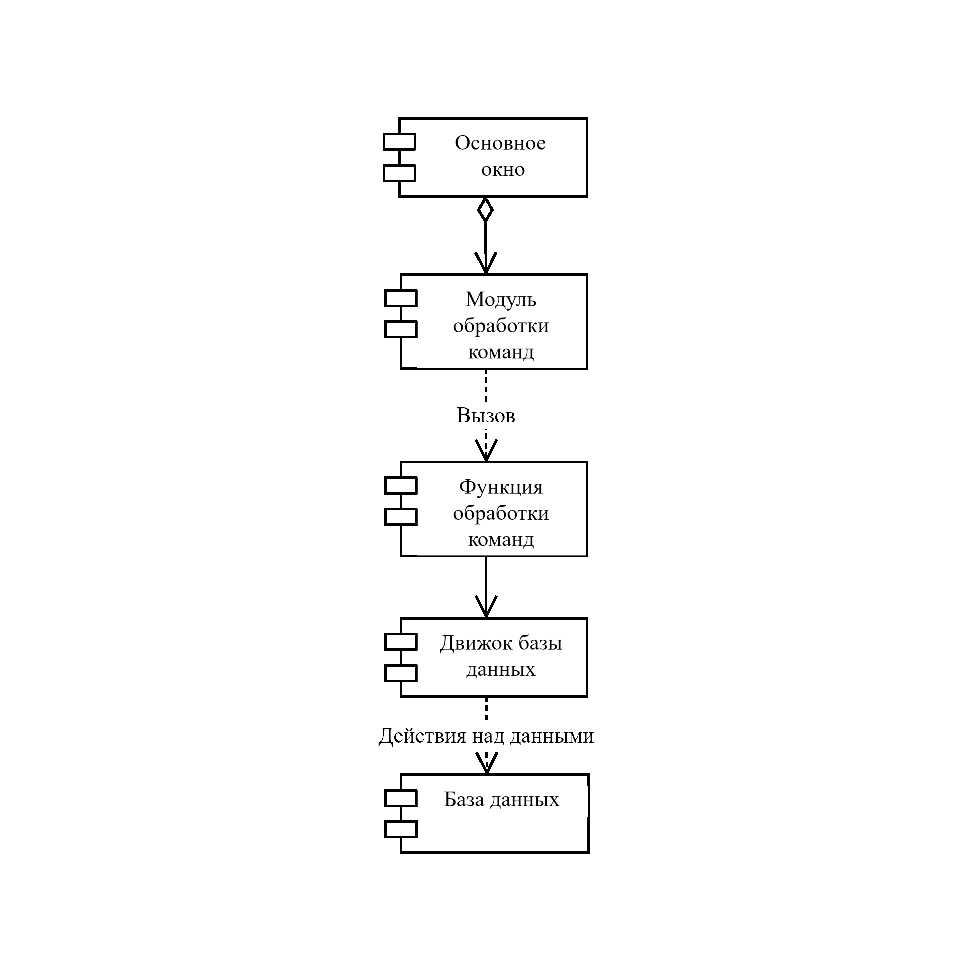
\includegraphics[width=1\linewidth]{images/svg_arch}
	\caption{Архитектура программной системы}
	\label{fig:arch}
\end{figure}

Программа разделена на следующие компоненты:
\begin{enumerate}
	\item Основное окно. Данный модуль реализует интерфейс программной системы.
	\item Модуль обработки команд. Данный модуль обрабатывает пользовательские команды и передаёт соответствующие инструкции в движок базы данных.
	\item Движок базы данных. Этот модуль отвечает за операции над данными в файле базы данных.
	\item Непосредственно сама база данных, представляющая собой .db файл с фиксированной структурой.
\end{enumerate}

\subsection{Архитектура базы данных}

Исходя из требований технического задания, программно-информационная система предназначена для работы с пользовательскими табличными структурами, которые хранятся на диске. Система реализует собственную модель хранения и управления данными средствами языка Python.

\subsubsection{Файл базы данных}

Файл базы данных в реализованной СУБД представляет собой бинарный файл фиксированной структуры, организованный на основе страничного подхода. Такой подход обеспечивает возможность масштабируемого хранения и упрощает работу с диском.

\paragraph{Структура файла}

Файл состоит из трёх основных областей:
\begin{enumerate}
	\item Заголовок файла (3 байта), который содержит информацию о текущем числе таблиц и указатель на первую свободную страницу.
	\item Метаданные таблиц (до 255 таблиц по 4358 байт). Каждая запись содержит название таблицы (до 16 символов); указатели на первую и последнюю страницы таблицы; размер одной записи таблицы в байтах; количество столбцов и описание каждого столбца (название длиной до 16 символов и тип данных).
	\item Страницы хранения данных (по 4096 байт). Каждая страница содержит заголовок (6 байт), содержащий указатель на следующую страницу и количество записей на странице; непосредственно данные -- записи таблицы.
\end{enumerate}

\paragraph{Типы данных}

Поддерживаются три типа данных:
\begin{itemize}
	\item integer -- целочисленный тип, 4 байта;
	\item float -- вещественный тип, 4 байта;
	\item string -- строковый тип, фиксированные 255 байт.
\end{itemize}

\paragraph{Страничная организация}

Каждая страница в файле имеет фиксированный размер в 4096 байт и используется для хранения записей определённой таблицы. Это позволяет организовывать данные в виде цепочек страниц (связный список), где каждая страница знает, какая следующая за ней. Конец списка обозначается специальной константой DEAD\_END, представленной как 0xFFFFFFFF.

Если при вставке записи текущая последняя страница таблицы не имеет достаточно места для новой записи, выделяется новая страница, которая прикрепляется к цепочке.

\subsubsection{Движок базы данных}

Движок базы данных реализует программную логику обработки данных и взаимодействия с бинарным файлом. Он состоит из набора методов класса Database, реализующих основные операции над таблицами и данными: создание таблиц, вставка, выборка, обновление и удаление.

\paragraph{Создание таблицы}

Метод create\_table позволяет создать новую таблицу с заданным именем и структурой. В процессе создания проверяется длина имени таблицы и названий столбцов; генерируется блок метаданных; производится запись в соответствующую область метаданных; выделяется новая страница под таблицу, если необходимо.

\paragraph{Удаление таблицы}

Метод drop\_table позволяет удалить указанную таблицу из базы данных. В процессе удаления полностью стираются все записи таблицы и её метаданные.

Освободившиеся страницы могут использоваться повторно при операциях создания таблиц и вставки данных.

\paragraph{Вставка данных}

Метод insert реализует логику вставки новой записи. Алгоритм включает в себя поиск нужной таблицы по имени; проверку типов данных и количества вставляемых значений; поиск последней страницы таблицы; вставку записи в свободное место либо аллокацию новой страницы при необходимости.

\paragraph{Выборка данных}

Метод select позволяет получить записи таблицы по заданному условию (фильтру). Возвращаются как данные, так и метаинформация о типах столбцов. Алгоритм включает в себя поиск таблицы и считывание метаданных; итерацию по цепочке страниц; распаковку записей и фильтрацию по переданному условию.

\paragraph{Обновление данных}

Метод update позволяет изменить существующие записи. Алгоритм включает в себя поиск таблицы и считывание метаданных; проверка корректности переданных значений; поиск всех записей, удовлетворяющих условию; перезапись выбранных записей на месте в бинарном файле.

\paragraph{Удаление данных}

Метод delete реализует удаление записей. В процессе удаления выполняется выборка всех записей с последующей фильтрацией; оставшиеся записи пакуются заново и перезаписываются в страницы; лишние страницы освобождаются.

Освобождённые после удаления данных страницы могут быть повторно использованы при операциях создания таблиц и вставки данных.

\subsection{Обработчик команд}

Обработчик команд является важным компонентом системы управления базой данных, обеспечивая взаимодействие пользователя с хранилищем данных через текстовые команды. Он интерпретирует пользовательский ввод, распознаёт тип действия и вызывает соответствующие методы движка базы данных. 

\subsubsection{Общий принцип работы}

Обработчик команд реализован в виде функции parse\_command, которая принимает строку с командой и объект базы данных. На первом этапе осуществляется предварительная обработка строки: строка разбивается на токены с использованием метода split(). Первый токен интерпретируется как ключевое слово действия -- create, drop, insert, select, delete или update. В зависимости от распознанного действия вызывается соответствующая логика обработки команды.

\subsubsection{Обработка условий where}

Для разбора логических выражений, указываемых в where-части команд, используется встроенный модуль ast (Abstract Syntax Tree). Это позволяет в качестве условий записывать логические выражения на синтаксисе Python. В условии допускается использование математических операций (+, -, *, /, **), операторов сравнения (>, <, >=, <=, ==, !=) и логических операторов (and, or, not). Выражения обрабатываются функцией eval\_node.

\subsubsection{Синтаксис SQL-команд}

\begin{enumerate}
	\item Создание базы данных: create database <название\_БД>.
	\item Создание таблицы: create table <имя\_таблицы> <столбец1> <тип1> <столбец2> <тип2> ... .
	\item Удаление таблицы: drop table <имя\_таблицы>.
	\item Вставка данных: insert into <имя\_таблицы> values <значение1> <значение2> ... .
	\item Выборка данных: select <столбцы|*> from <имя\_таблицы> [where <условие>].
	\item Удаление данных: delete from <имя\_таблицы> [where <условие>].
	\item Обновление данных: update <имя\_таблицы> set <столбец1> <значение1> ... [where <условие>].	
\end{enumerate}

\subsection{Проектирование пользовательского интерфейса}

На основании требований к пользовательскому интерфейсу, представленных в пункте 2.3.2 технического задания, был разработан графический интерфейс приложения.

На рисунке ~\ref{fig:interface} представлен макет рабочего окна программы. 

\begin{figure}[H]
	\centering
	\includegraphics[width=1\linewidth]{images/interface}
	\caption{Макет рабочего окна программы}
	\label{fig:interface}
\end{figure}

Макет содержит следующие элементы:
\begin{enumerate}
	\item Главное меню
	
	Главное меню реализовано на основе виджета tk.Menu и состоит из двух основных разделов:
	\begin{itemize}
		\item Select database -- вызывает окно выбора файла базы данных;
		\item Run -- команда запуска обработки пользовательского ввода, выполняющей анализ текста, введённого в поле SQL-команды, и выполнение соответствующих операций.
	\end{itemize}
	Меню охватывает основные действия, необходимые для работы пользователя с базой данных, и остаётся доступным вне зависимости от текущего состояния приложения.
	
	\item Область отображения таблиц
	
	Эта часть интерфейса занимает верхнюю половину окна и реализована с помощью контейнера tk.Frame и виджета ttk.Treeview, предназначенного для отображения табличных структур в виде древовидной таблицы с колонками. Таблица автоматически подстраивается под содержимое и заполняет всё доступное пространство. Для удобства просмотра добавлены горизонтальная и вертикальная полосы прокрутки.
	
	При проведении операций над данными интерфейс обновляется динамически, подставляя актуальные данные в таблицу.
	
	\item Поле ввода команд
	
	В нижней части окна находится текстовое поле tk.Text, предназначенное для ввода пользователем команд на SQL-подобном языке. Это основная точка взаимодействия между пользователем и программной системой.
	
	По нажатию пункта Run введённая команда передаётся в обработчик команд. Результат выполнения команды отображается либо в таблице, либо во всплывающем сообщении.
\end{enumerate}
